\documentclass[12pt]{standalone}

\usepackage{tikz}

\tikzset{real edge/.style={solid,very thick}}

\begin{document}
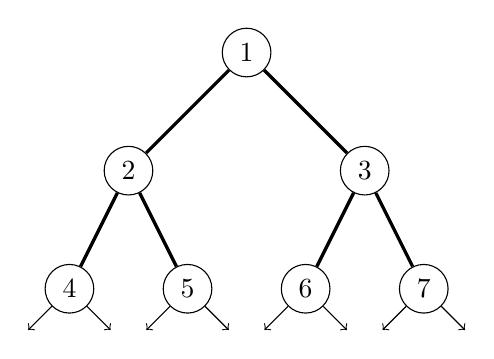
\begin{tikzpicture}

    \scoped[every node/.style={solid,thin,circle,draw}]
    \node (1) {1}
    child[real edge] {node (2) {2}
            child[real edge] {node (4) {4}}
            child[real edge] {node (5) {5}}}
    child[missing]
    child[real edge] {node (3) {3}
            child[real edge] {node (6) {6}}
            child[real edge] {node (7) {7}}};

            \foreach \node in {4, 5, 6, 7} {
                \draw[->] (\node.south west) -- ++(-0.3, -0.3);
            }
            \foreach \node in {4, 5, 6, 7} {
                \draw[->] (\node.south east) -- ++(0.3, -0.3);
            }

\end{tikzpicture}
\end{document}